\documentclass[11pt,a4paper]{article}
\usepackage[utf8]{inputenc}
\usepackage[T1]{fontenc}
\usepackage[spanish]{babel}
\usepackage{geometry}
\usepackage{graphicx}
\usepackage{booktabs}
\usepackage{amsmath}
\usepackage{hyperref}
\geometry{margin=2.4cm}
\title{Similaridad entre LLMs generadores: dos planos de medida\\
\large Cross-perplexity, embeddings, estilometría y rigidez estilística --- 87 generadores}
\author{miUrba2 --- experimento de fingerprints entre generadores}
\date{Septiembre 2026}

\begin{document}
\maketitle

\begin{abstract}
Presentamos un experimento de similaridad entre 87 modelos generadores de lenguaje,
evaluado con cuatro métricas independientes construidas sobre 256 quejas vecinales
generadas (3 escenarios por modelo): (1) \emph{cross-perplexity} con KLD/Jeffreys
derivados de logprobs exactas vía \texttt{prompt\_logprobs} parcheado en llama.cpp;
(2) similitud coseno entre centroides de embeddings con 7 jueces de 6 linajes;
(3) estilometría clásica (\emph{trigram-cosine delta} y perfiles POS/dependencias);
y (4) una sonda de \emph{rigidez estilística} (paráfrasis con un modelo común y
medida del drift). Las cuatro métricas convergen en el eje estilístico
($\rho$=0.38--0.83) y divergen de forma informativa en el eje semántico
($\rho_{\text{KLD,Emb}}$=+0.40), cuantificando la separación entre ``cómo escriben''
y ``qué escriben''. Validamos que las 7 cuantizaciones del mismo modelo producen
distancias triviales (validación), que los distills de la misma línea se agrupan,
y que la rigidez es una propiedad nueva y parcialmente independiente de la
distintividad.
\end{abstract}

\section{Infraestructura}
Los 87 generadores se despliegan como variantes \texttt{-xppl} en un gateway
\texttt{llama-swap} sobre 4$\times$RTX~3090: imagen Docker \texttt{llama-cpp-539f245-xppl}
(llama.cpp en el commit 539f245 con un parche que expone \texttt{prompt\_logprobs},
1 request por texto para la NLL completa del prompt). La generación es greedy
(temperature=0, penalizaciones neutras) lo que garantiza la diagonal exacta
($E{=}G \Rightarrow$ PPL$\approx$1). Los jueces de embedding se sirven con el mismo
binario en modo \texttt{/v1/embeddings} (6 linajes: Qwen3, Llama-3.1-NVIDIA,
Gemma-3 encoder, MiniLM-2021, LaBSE-2020, BERT-multilingüe-crudo-2018).

\section{Métricas}
\begin{enumerate}
\item \textbf{KLD/Jeffreys (distribucional).} $H(A,\text{text}_B)$ = NLL nats/token del
texto de $B$ bajo el evaluador $A$, condicionado al prompt de generación de $B$.
$\mathrm{KLD}[A][B] \approx \mathrm{KL}(P_B \| P_A) = H(A,\text{text}_B)-H(B,\text{text}_B)$;
$J[A][B]=\mathrm{KLD}[A][B]+\mathrm{KLD}[B][A]$ (simétrica).
\item \textbf{Embeddings (semántico).} Centroides por generador de los embeddings de
sus textos (formato de instrucción oficial de cada juez), similitud coseno,
fusión por media de z-scores del $1-\cos$ entre jueces.
\item \textbf{Estilometría (superficie y gramática).} \emph{Trigram-cosine delta}: top-1000
trigramas de caracteres, frecuencias relativas z-scoreadas, coseno (Salnikov \& Bonch 2025).
\emph{POS/dep delta}: perfiles POS y dependencias (spaCy es-core), coseno (Rosenfeld 2024).
\item \textbf{Rigidez (causal).} Paráfrasis forzada de cada texto con un rewriter común
(gemma-2-2b-it) y drift estilístico medido con CHRF-like (trigramas de caracteres).
Alta similitud original-rewrite = fingerprint ``invasivo'' (SSLA 2026, adaptado).
\end{enumerate}

\section{Resultados principales}
\subsection{Convergencia entre métricas}
\begin{table}[h]\centering
\begin{tabular}{lcccc}
\toprule
Spearman $\rho$ & KLD & Emb7 & Tri & POS\\
\midrule
KLD & --- & +0.40 & +0.38 & +0.25\\
Emb7 & +0.40 & --- & \textbf{+0.78} & +0.71\\
Tri & +0.38 & \textbf{+0.78} & --- & \textbf{+0.83}\\
POS & +0.25 & +0.71 & \textbf{+0.83} & ---\\
\bottomrule
\end{tabular}
\caption{Correlaciones triangulares sobre pares comunes (KLD limitado a 153 pares
de 18 generadores con diagonal; resto 3741 pares de 87).}
\end{table}

La estructura es la esperada: las tres métricas de \emph{estilo} (KLD, trigramas,
POS) convergen entre sí ($\rho$ 0.71--0.83 con los embeddings, que mezclan semántica
y estilo), y el KLD se distancia más de la métrica semántica pura. El eje
``cómo escriben'' está medido de tres formas independientes y coincide; el eje
``qué escriben'' (embedding) es complementario.

\begin{figure}[h]\centering
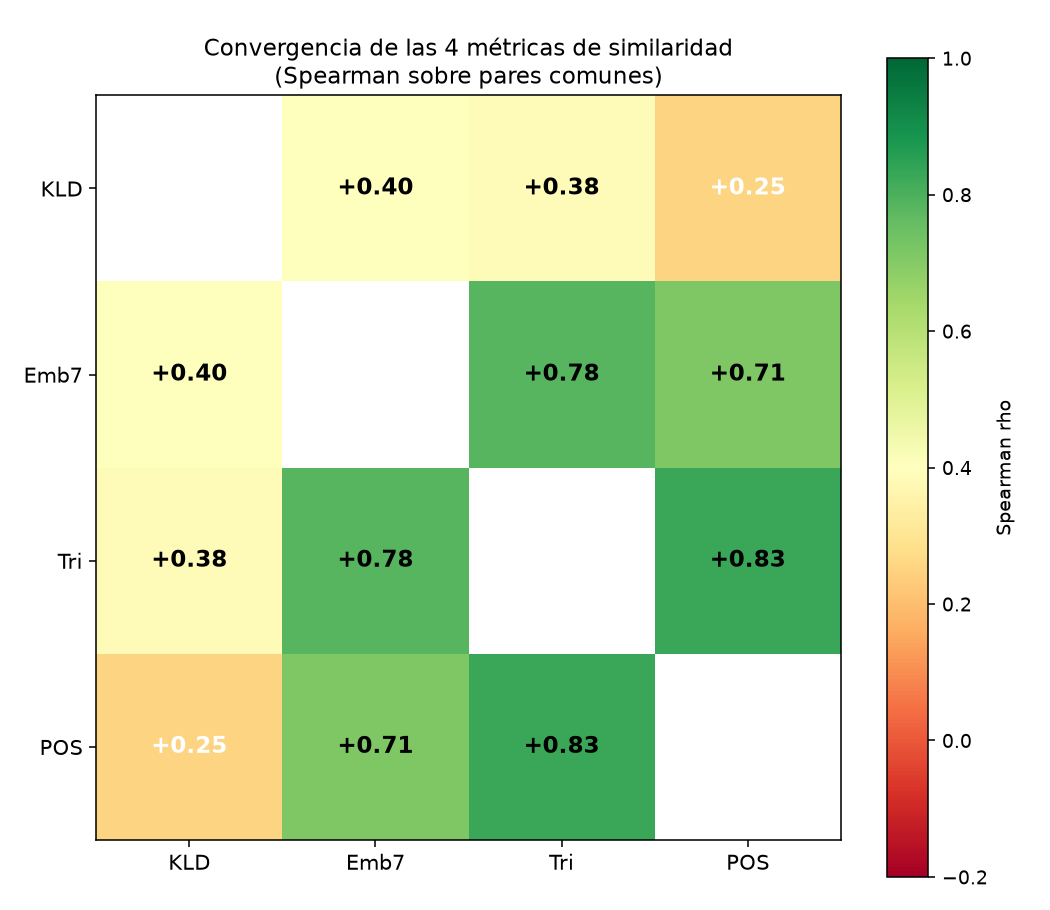
\includegraphics[width=0.72\textwidth]{fig_correlations_4metrics.png}
\caption{Heatmap de correlaciones entre las cuatro métricas.}
\end{figure}

\subsection{Validaciones internas}
Las 7 cuantizaciones de \texttt{qwen3.5-122b-a10b} (q3/q4, think/nothink) tienen
delta-trigram $\approx 0.000$ entre sí: el método resuelve ``mismo modelo, distinta
cuantización''. Los distills deepseek-r1 forman clanes (J$\leq$0.6), igual que la
familia falcon3 (0.53--0.64) y apertus (0.65) --- coherente con linajes de entrenamiento.

\subsection{Parejas extremas}
\textbf{Indistinguibles:} \texttt{agentica-deepcoder-14b} $\approx$
\texttt{deepseek-r1-distill-qwen-14b} (J=0.04).
\textbf{Más distantes:} \texttt{deepseek-r1-qwen-7b} $\leftrightarrow$ gemma-3-12b/27b
($J\approx$3.5--3.6). \textbf{Divergencias tipo}: gemma-2-2b $\leftrightarrow$
gemma-3-27b (contenido similar, estilo muy distinto: J=2.84 vs $D_{\text{emb}}$=0.73);
apertus-8b $\leftrightarrow$ deepseek-r1-32b (estilo parecido J=1.46, contenido
distinto $D_{\text{emb}}$=2.41).

\subsection{Rigidez estilística (87 generadores)}
Media CHRF=0.713, $\sigma$=0.150, rango [0.19, 0.94]. Los fingerprints más
\emph{invasivos}: pantheon-rp-8b (0.94), glm-4.5-air (0.93), deepseek-r1-32b (0.92),
llama-3.2-1b (0.91). Los más \emph{flexibles}: falcon3-1b (0.19), phi-4-reasoning-plus
(0.25), kimi-dev-72b (0.31). Correlación con la distintividad semántica: $\rho$=$-$0.25
--- propiedades \textbf{casi ortogonales}: un modelo puede tener estilo muy invasivo
pero contenido genérico, o viceversa.

\begin{figure}[h]\centering
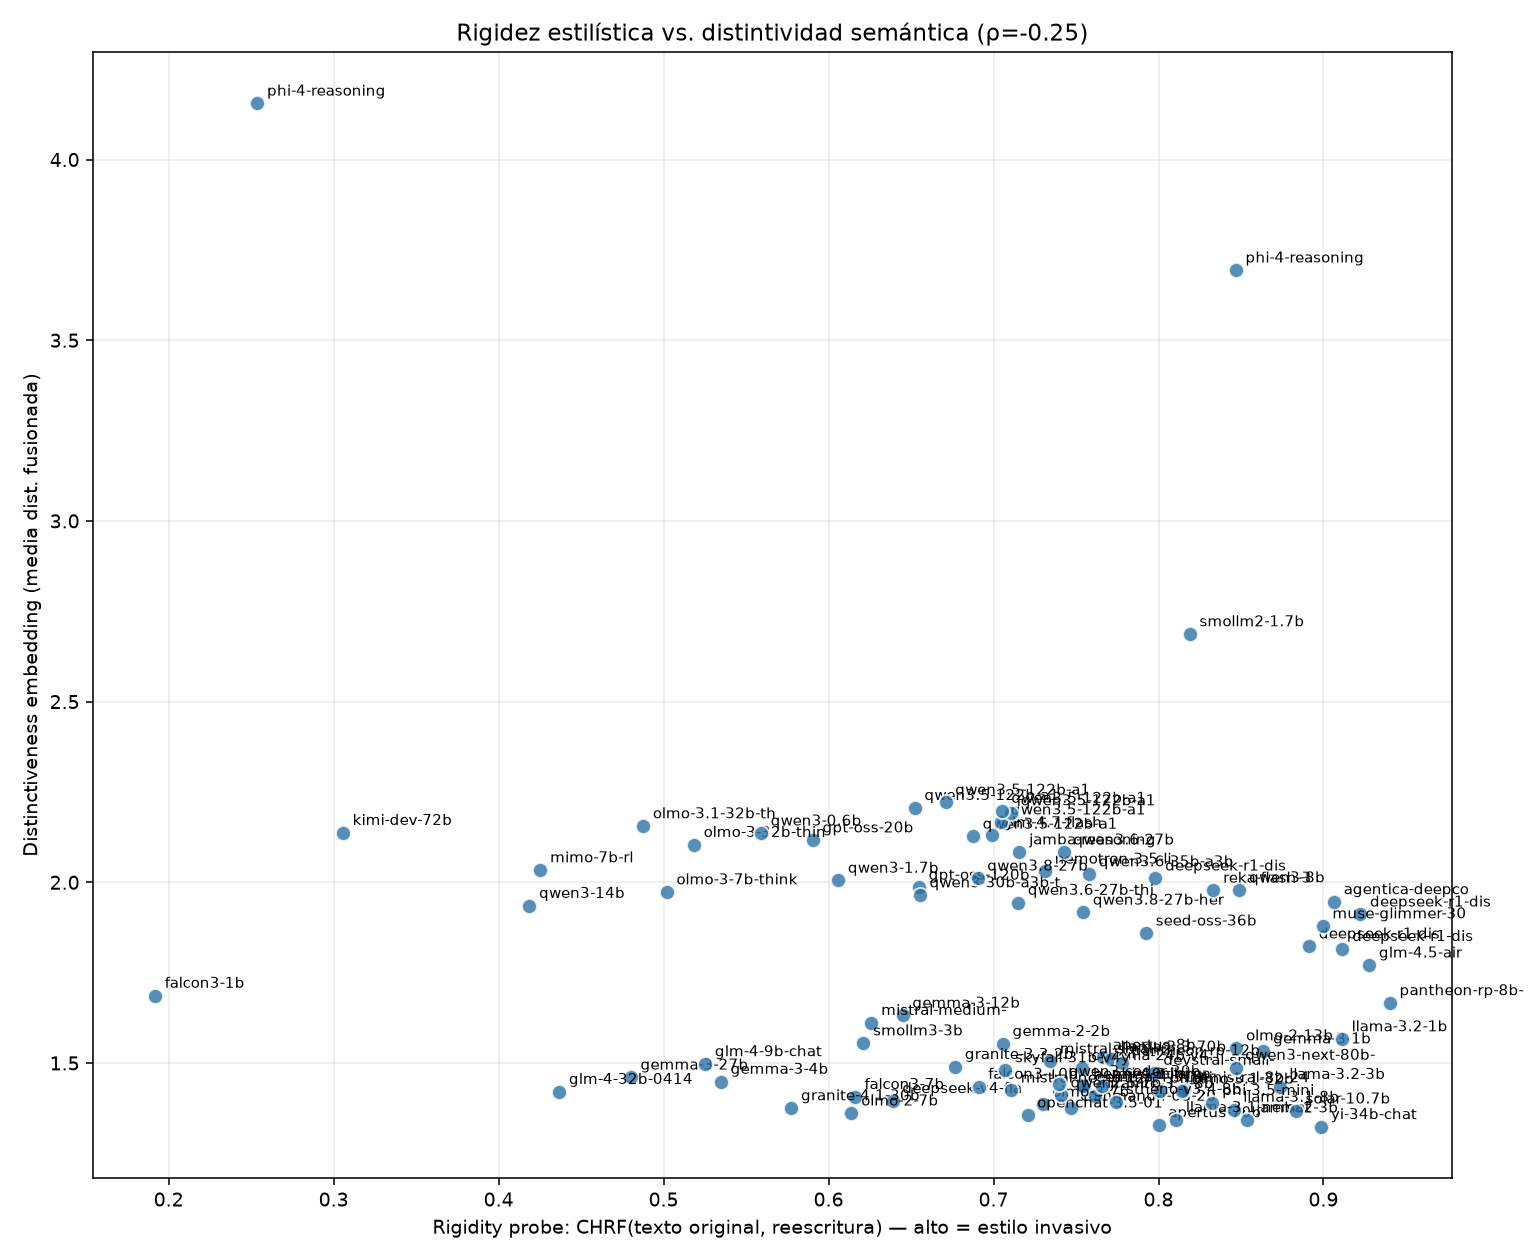
\includegraphics[width=0.78\textwidth]{fig_rigidity_vs_distinctiveness.png}
\caption{Rigidez estilística vs. distintividad semántica (87 generadores).}
\end{figure}

\begin{figure}[h]\centering
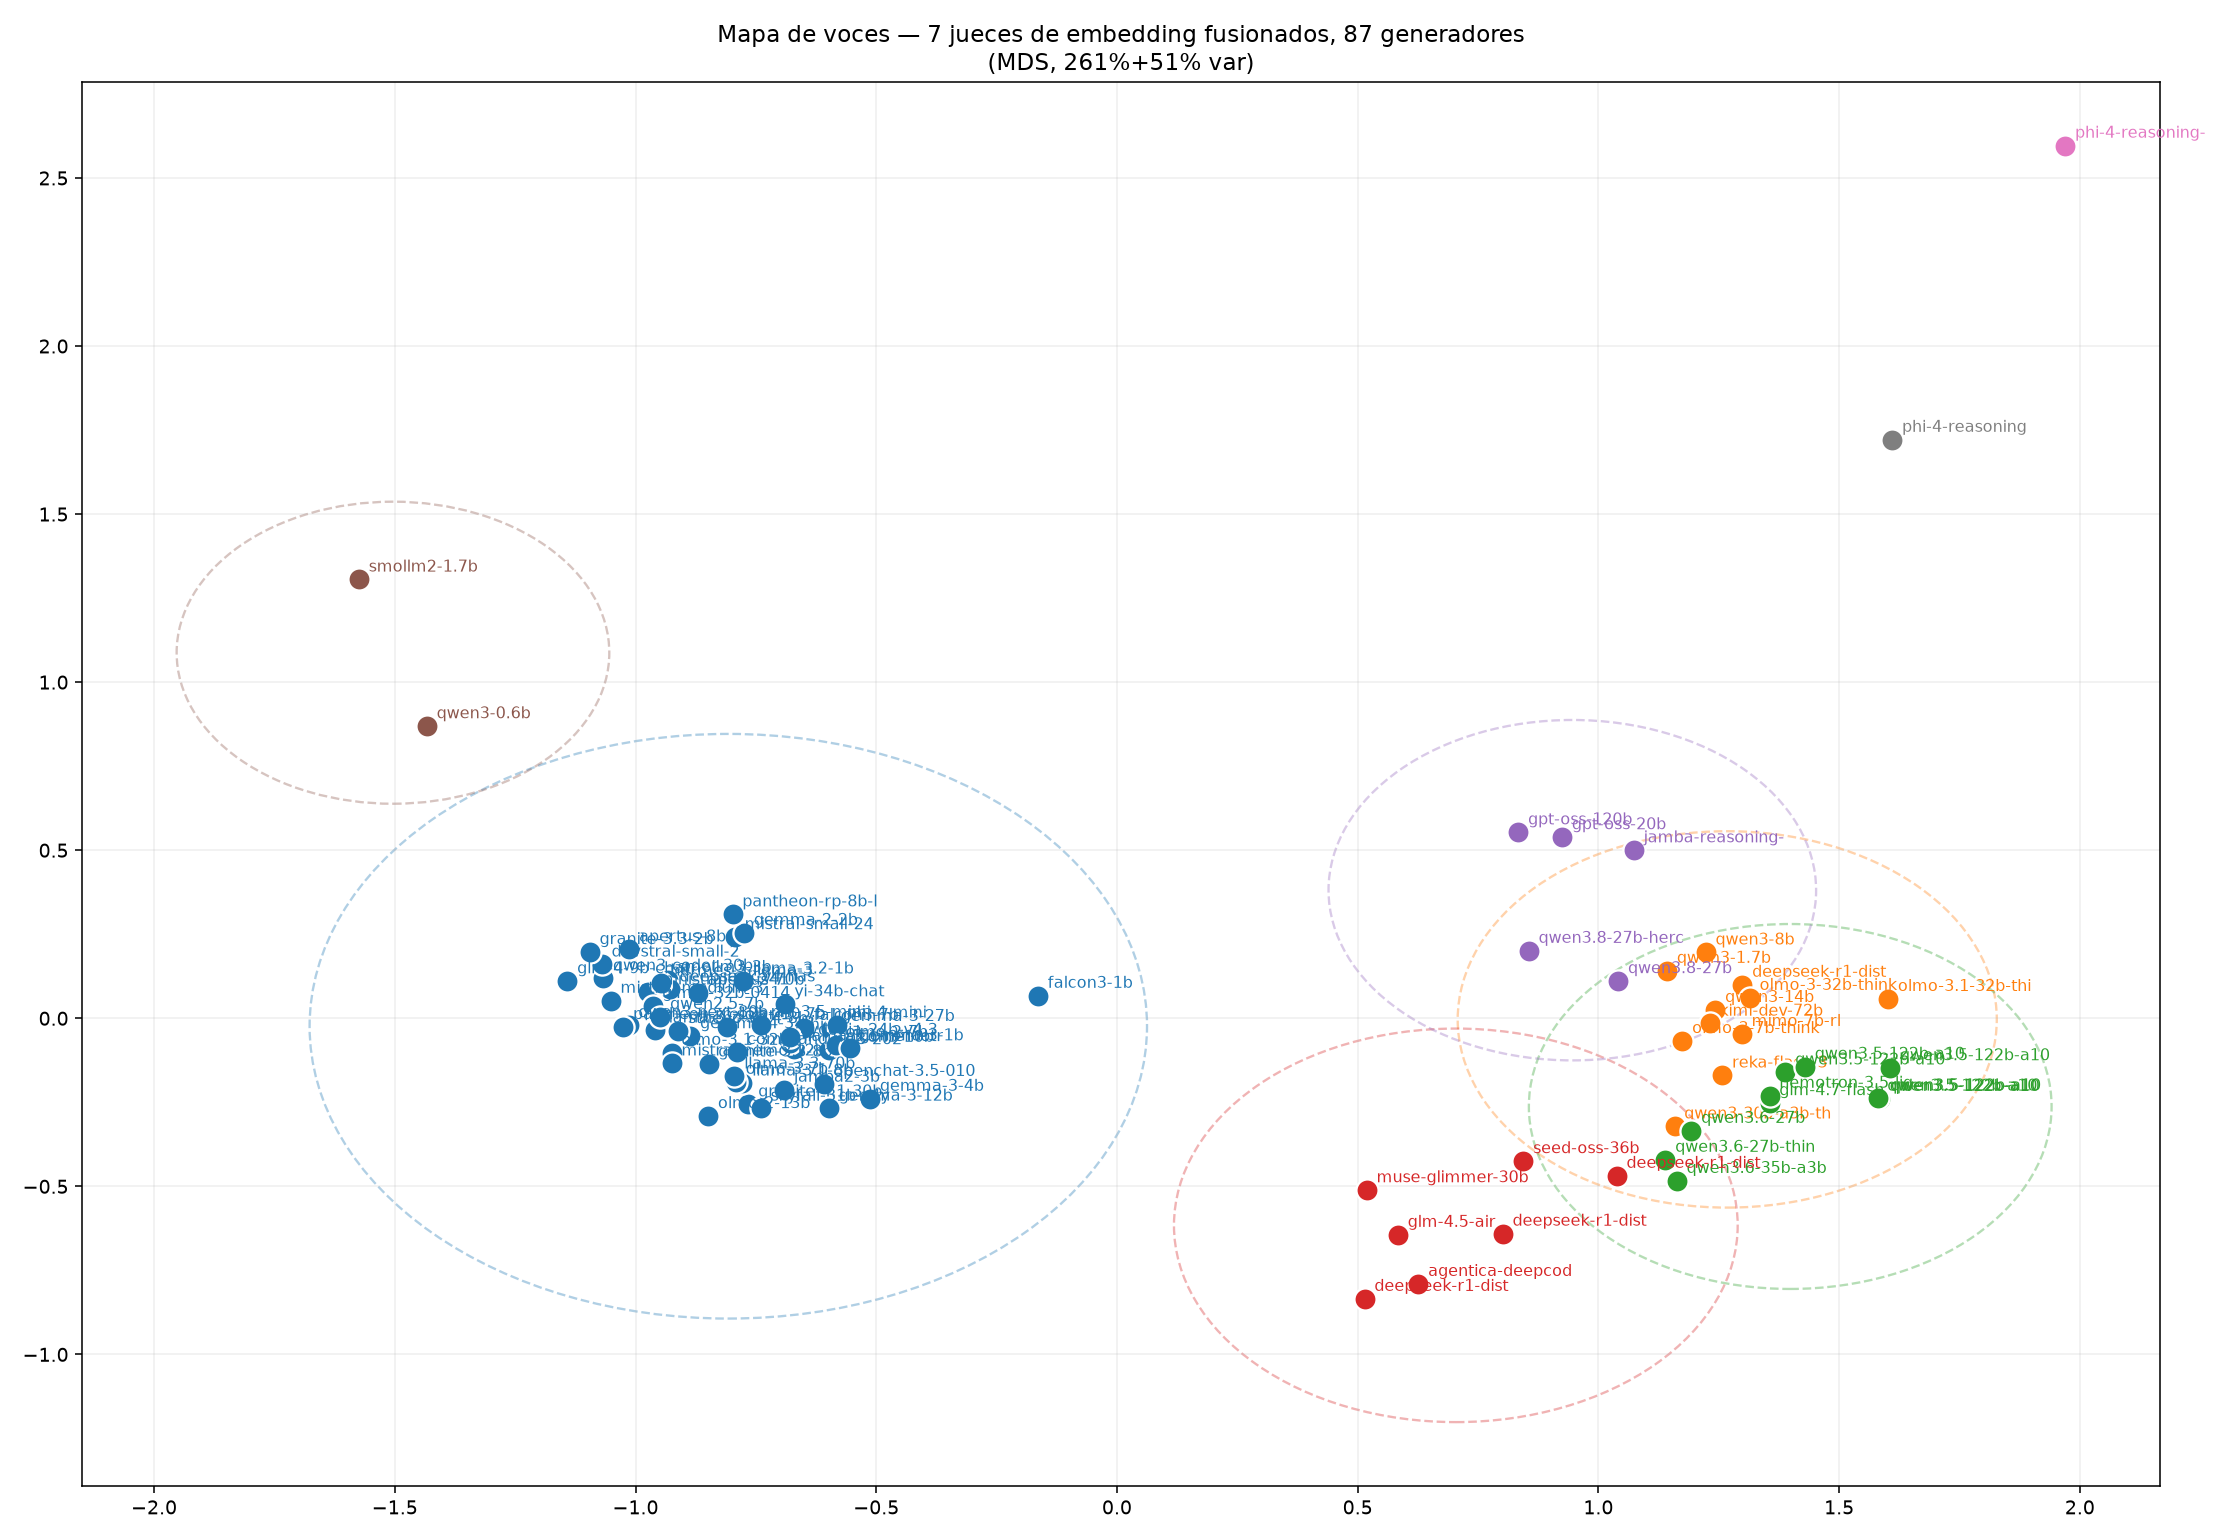
\includegraphics[width=0.95\textwidth]{mds_voces_embeddings_7j.png}
\caption{Mapa de voces: MDS de la distancia de embeddings fusionada (7 jueces), clusters K=8.}
\end{figure}

\section{Relación con la literatura}
Los resultados replican y extienden tres líneas: (a) \emph{LLM fingerprints} estilométricos
(McGovern et al.\ 2024, ``Your LLMs Are Leaving Fingerprints'': consistencia intra-familia
con caída de recall 0.01 intra-familia vs 0.62 inter-familia); (b) \emph{trigram-cosine delta}
(Salnikov \& Bonch-Osmolovskaya 2025: ARI 0.70 clustering no supervisado, superior a
clasificadores BERT); (c) \emph{style inertia} y rigidez (SSLA, ACL Findings 2026).
Nuestra contribución: la descomposición de la similaridad de generadores en dos planos
(distribucional/estilístico vs.\ semántico) cuantificada con correlaciones cruzadas sobre
un panel de 87 modelos en español, y la rigidez como tercer eje causal.

\section{Reproducibilidad}
Scripts en \texttt{eval/}: \texttt{cross\_perplexity\_unified.py} (matriz KLD por gateway),
\texttt{embed\_similarity.py} (7 jueces), \texttt{stylometry\_analysis.py} (E1/E2),
\texttt{rigidity\_probe.py} (E3), \texttt{final\_analysis.py} (correlaciones y figuras).
Datos en \texttt{eval/results/diversity/}: matrices por escenario, caches de generación,
plantillas de chat extraídas de GGUF (\texttt{extract\_chat\_template.py}).

\end{document}